\documentclass[pdf]{beamer}
\mode<presentation>{}
\usetheme{Dresden}
\usepackage{apalike}
\usepackage{graphicx}
\usepackage{subcaption}
\usepackage{pgfplotstable}
\usepackage{graphicx,psfrag}
\usepackage{mwe,tikz}\usepackage[percent]{overpic}
%% preamble
\title{Robust Computational Models for Water Waves}
\author{Jordan Pitt, Stephen Roberts and Christopher Zoppou \\ Australian National University}
\newcommand\solidrule[1][0.25cm]{\rule[0.5ex]{#1}{1pt}}
\newcommand\dashedrule{\mbox{\solidrule[2mm]\hspace{2mm}\solidrule[2mm]}}
\newcommand{\dotrule}[1]{%
	\parbox[]{#1}{\dotfill}}

\begin{document}
%% title frame
\section{Introduction}
\begin{frame}
\titlepage
\end{frame}
\begin{frame}{Outline of the Presentation}
	%Modelling Process
	%SWWE
	%Serre
	%My Work
	
%	\begin{itemize}
%		\item Water Wave Modelling
%		\item Robust Computational Models
%	\end{itemize}
\end{frame}

\section{Water Wave Modelling}
\begin{frame}{Modelling}
	%Picture Physical Process -> Mathematical Description -> Studying Mathematical Description (Numerical Solution)
	\begin{figure}
		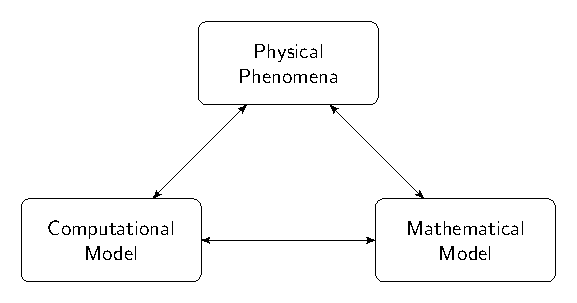
\includegraphics[width=\textwidth]{./Pics/ModelDiagrams/FlowChart.pdf}
	\end{figure}
\end{frame}
\begin{frame}{Physical Phenomena}
	%Picture Physical Process -> Mathematical Description -> Studying Mathematical Description (Numerical Solution)
	\begin{figure}
		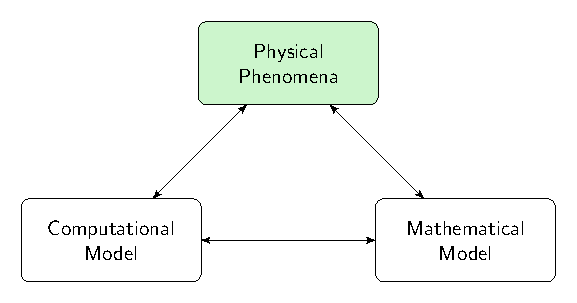
\includegraphics[width=\textwidth]{./Pics/ModelDiagrams/FlowChartHigh1G.pdf}
	\end{figure}
\end{frame}
\begin{frame}{Physical Phenomena: Water Waves}
	Water wave hazards:
		\begin{itemize}
			\item Tsunamis
			\item Storm Surges
			\item Rogue Waves
		\end{itemize}
	\smallskip
	Phenomena caused by water waves:
		\begin{itemize}
			\item Nutrient Transport
			\item Beach Erosion
			\item Breakup of Sea Ice
		\end{itemize}
\end{frame}
%Cool pictures
\begin{frame}{Typical Scenario}
	\begin{figure}
		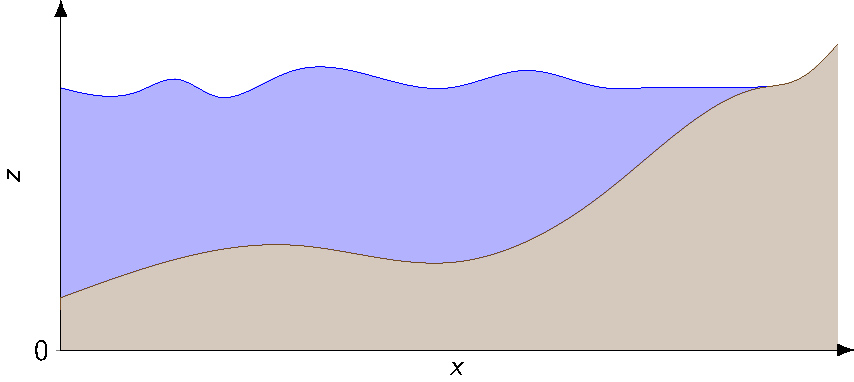
\includegraphics[width=\textwidth]{./Pics/WaterModelDiagrams/FressSurface.pdf}
	\end{figure}
\end{frame}


\subsection{Free Surface Flows}
\begin{frame}{Mathematical Model}
	%Picture Physical Process -> Mathematical Description -> Studying Mathematical Description (Numerical Solution)
	\begin{figure}
		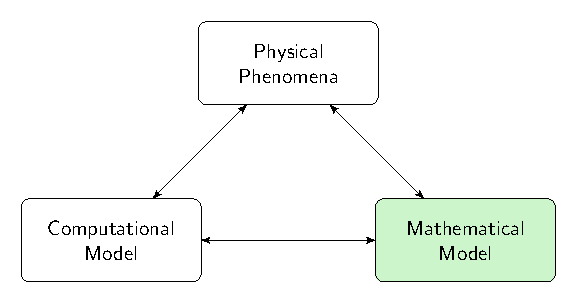
\includegraphics[width=\textwidth]{./Pics/ModelDiagrams/FlowChartHigh2G.pdf}
	\end{figure}
\end{frame}
\begin{frame}{Euler Model (Navier Stokes)}
	\begin{figure}
		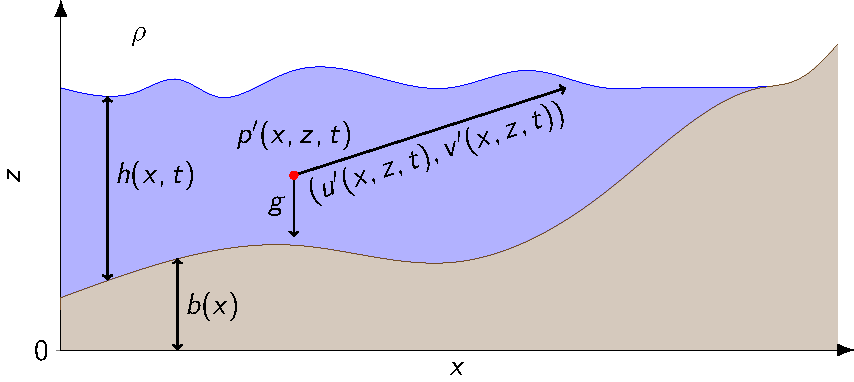
\includegraphics[width=\textwidth]{./Pics/WaterModelDiagrams/NavierStokes.pdf}
	\end{figure}
\end{frame}
\begin{frame}{Equations}
	Vectors:
	$\vec{u} = (u,v)$, $\quad \vec{g} = (0,-9.81 m/s^2)$
	\begin{align}
	& \text{Mass :} && {\color{gray} \frac{\partial \rho}{\partial t} + \rho} \nabla \cdot \vec{u} = 0 \\ \nonumber\\
	& \text{Momentum :} && \frac{\partial \vec{u}}{\partial t} + \nabla \cdot \left( \vec{u} \vec{u}^T\right) + \nabla p - \vec{g} = 0
	\end{align}	
\end{frame}
\begin{frame}{Pros and Cons}
	Pro:
	\begin{itemize}
		\item Models all water behaviour very well (density differences, viscosity, temperature negligible)
	\end{itemize}
	Con:
	\begin{itemize}
		\item Complex mainly due to number of terms $u$, $v$, $p$, $h$ and $b$. 
	\end{itemize}
\end{frame}
\begin{frame}{Computational Model}
\begin{figure}
	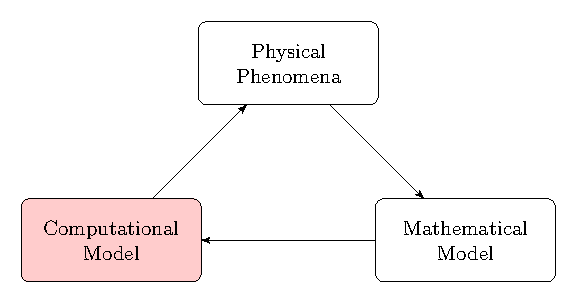
\includegraphics[width=\textwidth]{./Pics/ModelDiagrams/FlowChartHigh3.pdf}
\end{figure}
\end{frame}
\begin{frame}{Computational Model}
	\begin{itemize}
		\item Lots of good Computational Models for the Euler equations
		\item Computational Models only efficient and accurate over scale of metres
		\item We are interested in phenomena over the scale of kilometres to hundreds of kilometres
	\end{itemize}
	Require a different Mathematical Model to efficiently model water over the large extent of physical processes we are interested in. To do this we must reduce the number of quantities.
\end{frame}


\subsection{Shallow Water Wave Model}
\begin{frame}{Mathematical Model}
	%Picture Physical Process -> Mathematical Description -> Studying Mathematical Description (Numerical Solution)
	\begin{figure}
		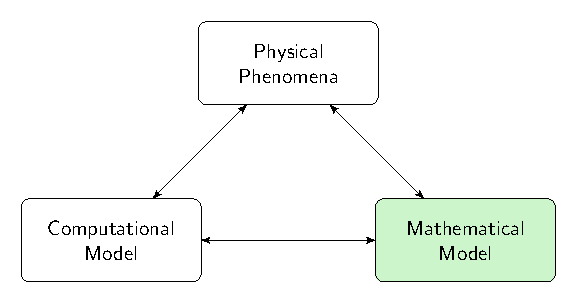
\includegraphics[width=\textwidth]{./Pics/ModelDiagrams/FlowChartHigh2G.pdf}
	\end{figure}
\end{frame}
\begin{frame}{Shallow Water Wave Model}
	\begin{figure}
		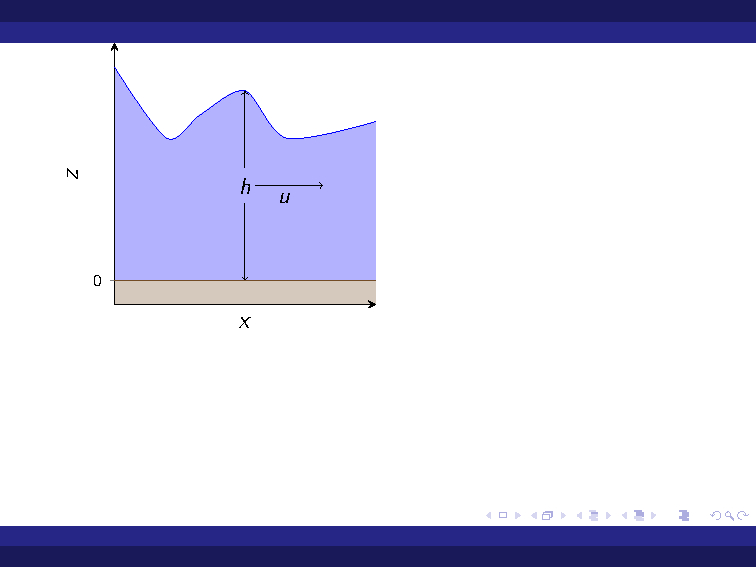
\includegraphics[width=\textwidth]{./Pics/WaterModelDiagrams/SWWE.pdf}
	\end{figure}
\end{frame}
\begin{frame}{Assumptions}
	\begin{itemize}
		\item $u(x,z,t)$ constant in $z$
		\item $v(x,z,t) = 0$
		\item $p(x,z,t) = g\left[ \left(h(x,t) - b(x)\right) - z\right]$
	\end{itemize}
\end{frame}
\begin{frame}{Equations}
	\begin{align}
	&\frac{\partial h}{\partial t} + \frac{\partial }{\partial x}\left( uh\right) = 0 \\ \nonumber \\
	&\frac{\partial u h}{\partial t} + \frac{\partial }{\partial x}\left( u^2h + \frac{1}{2}gh^2\right) + gh\frac{\partial b}{\partial x} = 0
	\end{align}
\end{frame}
\begin{frame}{Pros and Cons}
	Pro:
	\begin{itemize}
		\item Far simpler than the Euler equations
		\item Models waves with long wavelengths very well 
		\item Show good agreement with experimental results
	\end{itemize}
	Cons:
	\begin{itemize}
		\item No dispersion
		\item Poor model for short waves 
	\end{itemize}
\end{frame}
\begin{frame}{Computational Model}
		\begin{figure}
			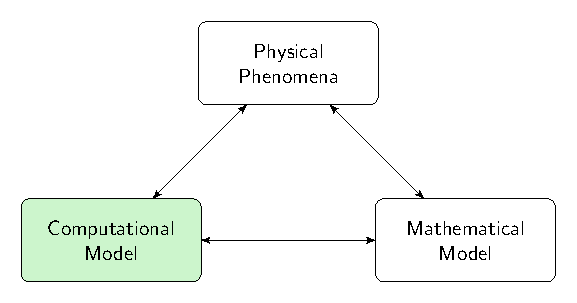
\includegraphics[width=\textwidth]{./Pics/ModelDiagrams/FlowChartHigh3G.pdf}
		\end{figure}
\end{frame}
\begin{frame}{Finite Volume Method}
	\begin{figure}
		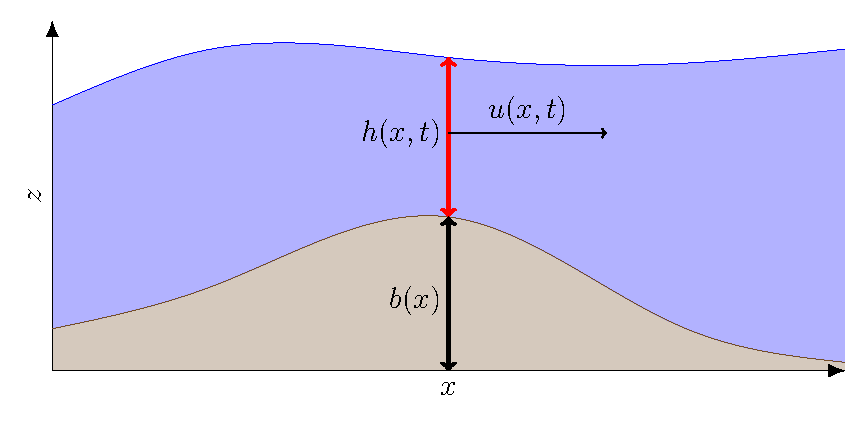
\includegraphics[width=\textwidth]{./Pics/FVMpicture/Problem.pdf}
	\end{figure}
\end{frame}
\begin{frame}{Equations}
	\begin{align}
	&\frac{\partial h}{\partial t} + \frac{\partial }{\partial x}\left( uh\right) = 0 \\ \nonumber \\
	&\frac{\partial u h}{\partial t} + \frac{\partial }{\partial x}\left( u^2h + \frac{1}{2}gh^2\right) + gh\frac{\partial b}{\partial x} = 0
	\end{align}
	
	General Conservation Form with Source Term
	\begin{equation}
	\frac{\partial q}{\partial t} + \frac{\partial f(q)}{\partial x} + s(q) = 0
	\end{equation}
\end{frame}
\begin{frame}{Cell Discretisation}
	\begin{figure}
		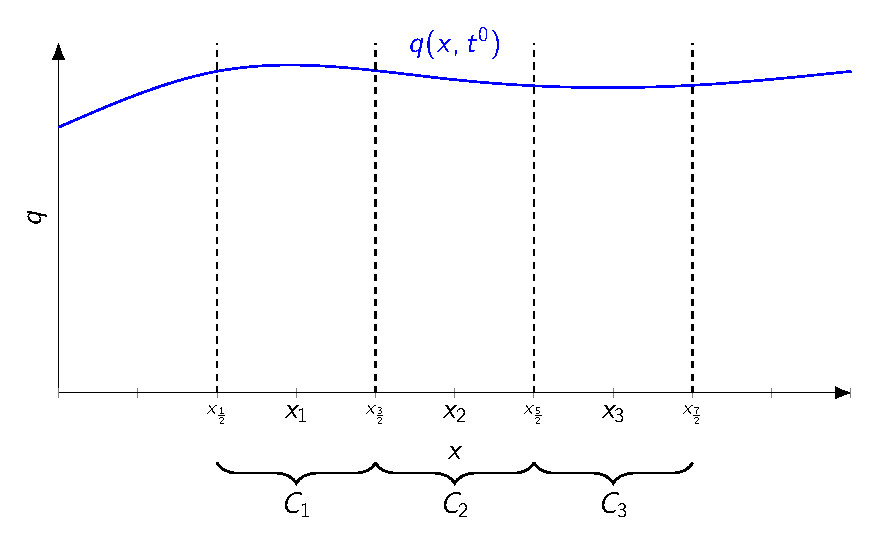
\includegraphics[width=\textwidth]{./Pics/FVMpicture/Cells.pdf}
	\end{figure}
\end{frame}
\begin{frame}{Cell Integration}
		\begin{equation*}
		\frac{\partial q}{\partial t} + \frac{\partial f(q)}{\partial x} + s(q) = 0
		\end{equation*}
		\begin{equation*}
		\frac{\partial}{\partial t} \int_{C_j} q \; dx + \left[f(q(x_{j+1/2},t)) - f(q(x_{j-1/2},t))  \right] + \int_{C_j} s(q) \; dx  = 0
		\end{equation*}
		\begin{equation*}
		\bar{q}(x_j,t)= \int_{C_j} q(x,t) \; dx
		\end{equation*}
		\begin{equation*}
		\frac{\partial}{\partial t} \bar{q}(x_j,t) + \left[f(q(x_{j+1/2},t)) - f(q(x_{j-1/2},t))  \right] + \int_{C_j} s(q) \; dx  = 0
		\end{equation*}
\end{frame}
\begin{frame}{Fluxes}
	\begin{figure}
		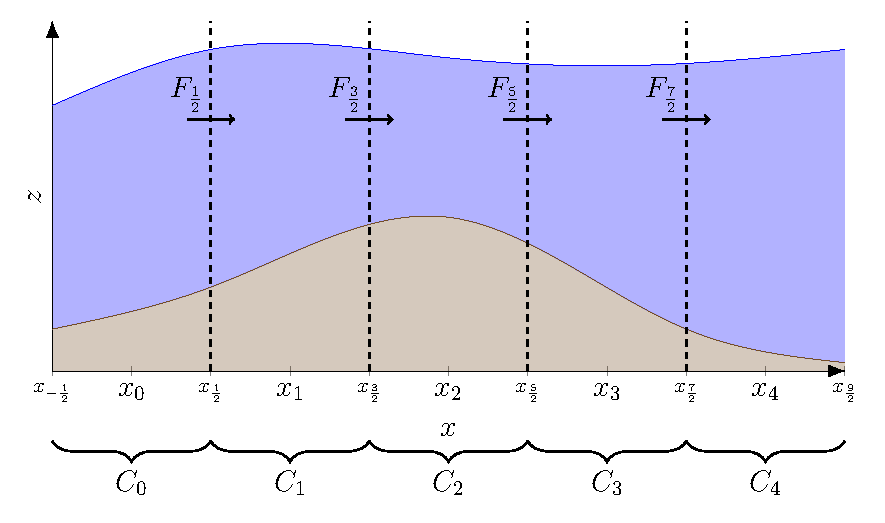
\includegraphics[width=\textwidth]{./Pics/FVMpicture/Fluxes.pdf}
	\end{figure}
\end{frame}
\begin{frame}{Time Integration}
	
	\begin{equation*}
	\frac{\partial}{\partial t} \bar{q}(x_j,t) + \left[f(q(x_{j+1/2},t)) - f(q(x_{j-1/2},t))  \right] + \int_{C_j} s(q) \; dx  = 0
	\end{equation*}
	
	\begin{equation}
	F_{j \pm 1/2} = \int_{t^n}^{t^{n+1}} f(q(x_{j\pm,1/2},t)) \; dt
	\end{equation}
  
	\begin{equation}
	\left[\bar{q}(x_j,t^{n+1}) - \bar{q}(x_j,t^n)\right]+ \left[F_{j + 1/2} - F_{j - 1/2} \right] +  \int_{t^n}^{t^{n+1}} \int_{C_j} s(q) \, dx \, dt = 0
	\end{equation}
\end{frame}
\begin{frame}{Source Terms}
	\begin{figure}
		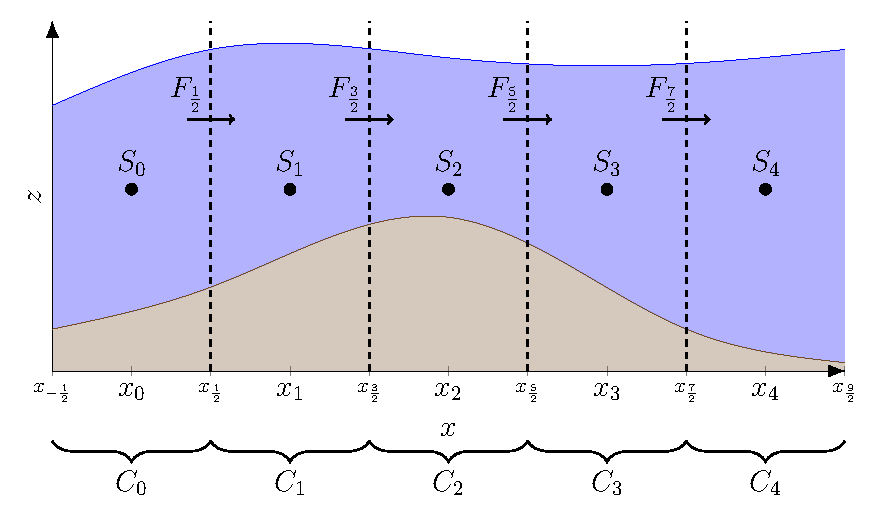
\includegraphics[width=\textwidth]{./Pics/FVMpicture/ALL.pdf}
	\end{figure}
\end{frame}
\begin{frame}{Update Formula}
	\begin{equation}
	\left[\bar{q}(x_j,t^{n+1}) - \bar{q}(x_j,t^n)\right]+ \left[F_{j + 1/2} - F_{j - 1/2} \right] +  \int_{t^n}^{t^{n+1}} \int_{C_j} s(q) \, dx \, dt   = 0
	\end{equation}
	
	\begin{equation}
	S_{j} = \int_{t^n}^{t^{n+1}} \int_{C_j} s(q) \; dx
	\end{equation}
	
	\begin{equation}
	\left[\bar{q}(x_j,t^{n+1}) - \bar{q}(x_j,t^n)\right]+ \left[F_{j + 1/2} - F_{j - 1/2} \right] +  S_j  = 0
	\end{equation}
	
		\begin{equation}
		\bar{q}(x_j,t^{n+1})  = \bar{q}(x_j,t^n) -  \left[F_{j + 1/2} - F_{j - 1/2} \right] -  S_j
		\end{equation}
	
	
\end{frame}
\begin{frame}{ANUGA}
	\begin{itemize}
		\item 1999 : Stephen Roberts and Chris Zoppou Paper solving SWWE
		\item 2004 : ANUGA development begins originally focusing on storm surges
		\item 2005 : ANUGA refocused to tsunamis
		\item 2006 : ANUGA has first public release
	\end{itemize}
\end{frame}


\begin{frame}{Pros and Cons}
	Pros
	\begin{itemize}
	\item Efficient, robust and accurate computational model based on the SWWE
	\end{itemize}
	Cons
	\begin{itemize}
	\item No dispersion because of the SWWE
	\item SWWE not valid for shorter wavelengths
	\end{itemize}
\end{frame}

\begin{frame}{Outcome}
 New Project at the ANU to build computational models from dispersive mathematical models
\end{frame}
%mention previous work of ANU


\subsection{Serre Model}
\begin{frame}{Mathematical Model}
	%Picture Physical Process -> Mathematical Description -> Studying Mathematical Description (Numerical Solution)
	\begin{figure}
		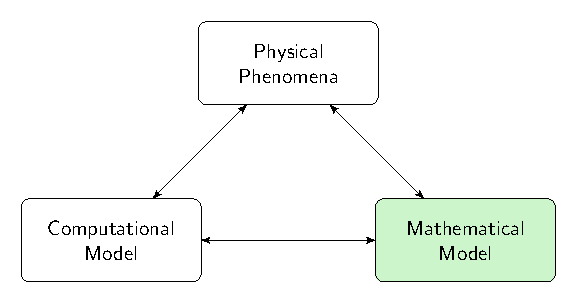
\includegraphics[width=\textwidth]{./Pics/ModelDiagrams/FlowChartHigh2G.pdf}
	\end{figure}
\end{frame}
\begin{frame}{Serre Model}
	\begin{figure}
		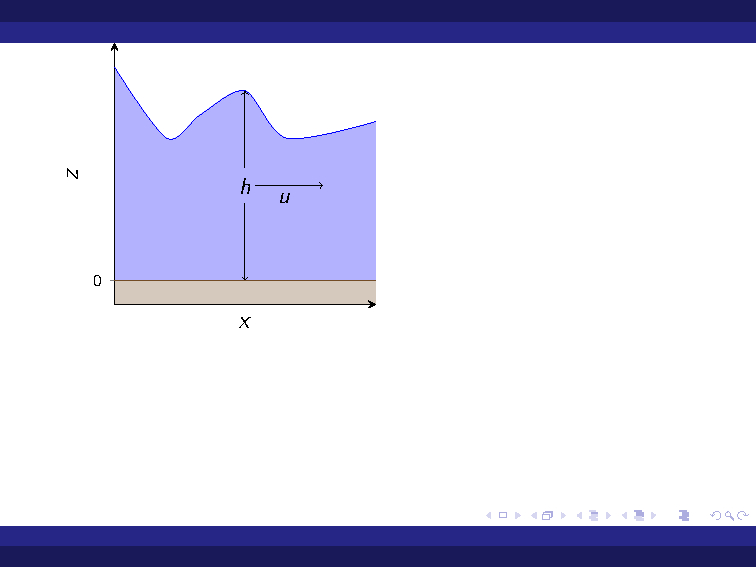
\includegraphics[width=\textwidth]{./Pics/WaterModelDiagrams/SWWE.pdf}
	\end{figure}
\end{frame}
\begin{frame}{Assumptions}
	\begin{itemize}
		\item $u(x,z,t)$ constant in $z$
		\item $v(x,z,t) = u\frac{\partial b}{\partial x} - (z - b)\frac{\partial b}{\partial x}$
		\item $p(x,z,t) = g\xi  + \xi \Psi + \frac{1}{2} \xi \left(2h - \xi\right) \Phi$
	\end{itemize}
\end{frame}
\begin{frame}{Equations}
	\begin{subequations}
		\begin{align*}
		&\frac{\partial h}{\partial t} + \dfrac{\partial (uh)}{\partial x} = 0,  \\ \\
		&\dfrac{\partial (uh)}{\partial t} + \dfrac{\partial}{\partial x} \left ( u^2h + \dfrac{gh^2}{2} + \dfrac{h^2}{2}{ \color{red}\Psi } + \dfrac{h^3}{3}{ { \color{blue} \Phi } }  \right )  +  \dfrac{\partial b}{\partial x} \left (gh +   h { \color{red}\Psi } + \dfrac{h^2}{2}{ { \color{blue} \Phi } }  \right ) = 0
		\end{align*}
	\end{subequations}
	with
		\begin{align*}
		&{ \color{red}\Psi }  = \dfrac{\partial b}{\partial x}\left(\dfrac{\partial u}{\partial t} + u\dfrac{\partial u}{\partial x} \right)  + u^2\dfrac{\partial^2 b}{\partial x^2}, \\&
		{ \color{blue} \Phi }  = \dfrac{\partial u }{\partial x} \dfrac{\partial u}{\partial x} -u \dfrac{\partial^2 u}{\partial x^2}  - \dfrac{\partial^2 u}{\partial x \partial t} .
		\end{align*}
\end{frame}
\begin{frame}{Pros and Cons}
	Pro:
	\begin{itemize}
		\item Far simpler than the Euler equations
		\item Maintains good model for long wavelength waves and extends our range of applicability to shorter wavelengths
		\item Has dispersion
		\item Considered one of the most appropriate models of water waves up to breaking
	\end{itemize}
	Cons:
	\begin{itemize}
		\item More complicated than the SWWE due to extra terms
		\item No well developed, efficient Robust Computational Models for three dimensional flows over complex geometries. 
	\end{itemize}
\end{frame}
\begin{frame}{Computational Model}
	%Picture Physical Process -> Mathematical Description -> Studying Mathematical Description (Numerical Solution)
	\begin{figure}
		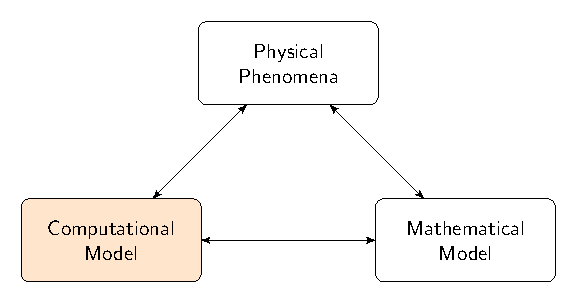
\includegraphics[width=\textwidth]{./Pics/ModelDiagrams/FlowChartHigh3O.pdf}
	\end{figure}
\end{frame}
\begin{frame}{Problem 1: Not in Conservative Form with Source Term}
	Recall:
	General Conservation Form with Source Term
	\begin{equation}
	\frac{\partial q}{\partial t} + \frac{\partial f(q)}{\partial x} + s(q) = 0
	\end{equation}
	Serre Equations:
	\begin{subequations}
		\begin{align*}
		&\frac{\partial h}{\partial t} + \dfrac{\partial (uh)}{\partial x} = 0,  \\ \\
		&\dfrac{\partial (uh)}{\partial t} + \dfrac{\partial}{\partial x} \left ( u^2h + \dfrac{gh^2}{2} + \dfrac{h^2}{2}{ \color{red}\Psi } + \dfrac{h^3}{3}{ { \color{blue} \Phi } }  \right )  +  \dfrac{\partial b}{\partial x} \left (gh +   h { \color{red}\Psi } + \dfrac{h^2}{2}{ { \color{blue} \Phi } }  \right ) = 0
		\end{align*}
	\end{subequations}
	with ${ \color{red}\Psi } $ and ${ \color{blue} \Phi } $ containing temporal derivatives of $u$
	
\end{frame}
\begin{frame}{Previous Work}
	\begin{itemize}
		\item 2014: Chris Zoppou's PhD thesis \\
			Demonstrated Computational Model for the Serre equations with varying bathymetry in 1D.
		\item 2014: My Honours thesis \\
			Independent reproduction of Chris's work
	\end{itemize}
	Open problems:
	\begin{itemize}
		\item Are solutions in the presence of steep gradient correct?
		\item Solution in the presence of dry beds
		\item Extension to 3D flows
	\end{itemize}	
\end{frame}



\section{Robust Computational Model}
%Goal of thesis to develop numerical method that can handle dry beds and steep gradients using FEM and FVM

\begin{frame}{Thesis Goals}
	Answer these open problems:
	\begin{itemize}
		\item Are solutions in the presence of steep gradient correct?
		\item Solution in the presence of dry beds
		\item Extension to 3D flows
	\end{itemize}
	Technique: Develop a numerical method for the 2D Serre equations with a Finite Volume method at its core that can readily be extended to 3D flows and is well validated for dry beds and steep gradients. 
\end{frame}

\subsection{Steep Gradients in the Flow}
%What was known
%Previous Work
%Improvements
\begin{frame}
\end{frame}


\subsection{Dry Beds}
%What was known
%Previous Work
%Improvements
\begin{frame}
\end{frame}

\end{document}